\chapter{\ifproject%
\ifenglish Project Structure and Methodology\else โครงสร้างและขั้นตอนการทำงาน\fi
\else%
\ifenglish Project Structure\else โครงสร้างของโครงงาน\fi
\fi
}


\makeatletter

% \renewcommand\section{\@startsection {section}{1}{\z@}%
%                                    {13.5ex \@plus -1ex \@minus -.2ex}%
%                                    {2.3ex \@plus.2ex}%
%                                    {\normalfont\large\bfseries}}

\makeatother
%\vspace{2ex}
% \titleformat{\section}{\normalfont\bfseries}{\thesection}{1em}{}
% \titlespacing*{\section}{0pt}{10ex}{0pt}

\section{โครงสร้างการทดลอง}

หลังจากกำหนดขอบเขตและหัวข้อโครงงาน และใช้แนวคิดการทดลองตามที่กลุ่มเราได้ว่าแผนกันโดยการขั้นตอนดังรูป ที่ 3.1

\begin{figure}[h!]
  \begin{center}
    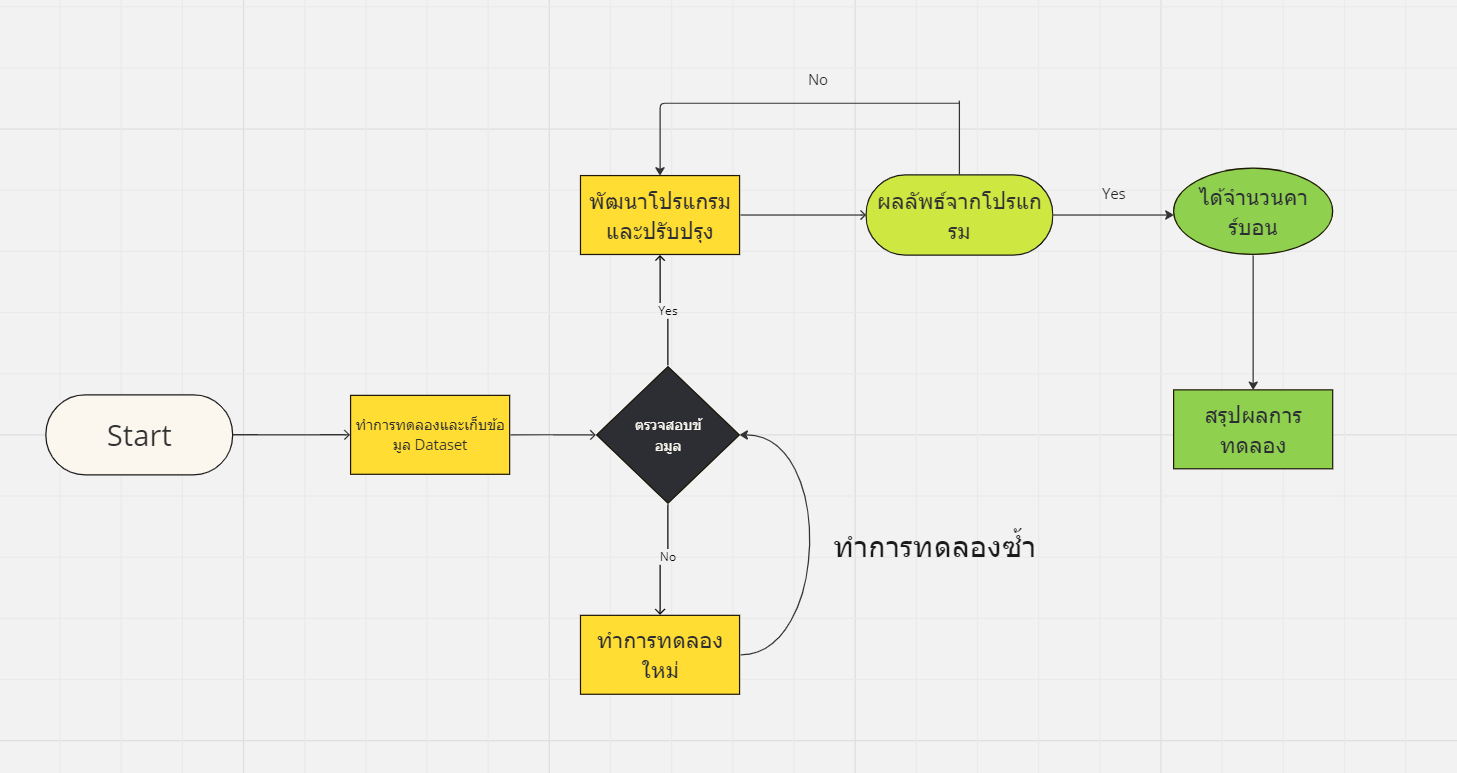
\includegraphics[width=\textwidth]{3_1.png}
  \end{center}
  \caption[Poem]{}
\end{figure}

\section{ขอบเขตการใช้งานระบบของผู้ใช้}

ระบบจะแบ่งผู้ใช้ออกเป็น 3 กลุ่มหลักๆ ได้แก่

\begin{enumerate}
  \item {อาจารย์ ครู}
  \item {บุคคลทั่วไปที่สนใจการทดลอง}
  \item {นักเรียน นักศึกษา}
\end{enumerate}

\subsection{อาจารย์ ครู}

\hspace{0.5 cm}โปรแกรมเราเหมาะสมสำหรับอาจารย์ หรือคุณครูที่กำลังสอนเกี่ยวกับการเกิดปฏิกิริยาอีมัลชั่นของก๊าซ \newline
คาร์บอน เพื่อจะแสดงจำนวนก๊าซคาร์บอนให้การทดลอง

\subsection{บุคคลทั่วไปที่สนใจการทดลอง}

\hspace{0.5 cm}บุคคลทั่วไปที่สนใจการทดลอง ที่สนใจในการทดลองหรือชอบความท้าทายในการทดลองเกี่ยวกับการผสม 
ก๊าซคาร์บอนกับก๊าซต่างๆ ในปฏิกิริยาอีมัลชั่น โดยสามารถนับจำนวนคาร์บอนที่มีรูปทรงต่างๆ จากโปรแกรมที่เราจะได้พัฒนาขึ้นมา

\subsection{นักเรียน นักศึกษา}

\hspace{0.5 cm}นักเรียน นักศึกษา ที่กำลังเรียนรู้เกี่ยวกับการเกิดอีมัลชั่นได้ โดยการผสมก๊าซคาร์บอนกับก๊าซต่างแล้วนับ จำนวนคาร์บอนที่เกิดขึ้นมาบันทึกเป็นกราฟทดลองได้ เช่นการทดลอง ก๊าซคาร์บอนกับก๊าซไนโตรเจน

ซึ่งขอบเขตการใช้งานระบบของผู้ใช้ อาจจะมีเพิ่มในภายหลัง ถ้ากลุ่มเราสามารถพัฒนาให้นับจำนวนก๊าซชนิดอื่นได้

\section{การเก็บข้อมูลการทดลอง และ การนับจำนวน}
หลังจากเราได้ทำการทดลองเสร็จแล้ว เราจะเก็บข้อมูลและนับจำนวนคาร์บอน ไม่ว่ารูปทรงจะเป็นอย่างไร \newline
ที่เราทดลองได้ ดังรูปตัวอย่างที่ 3.3

\begin{figure}[h!]
  \begin{center}
    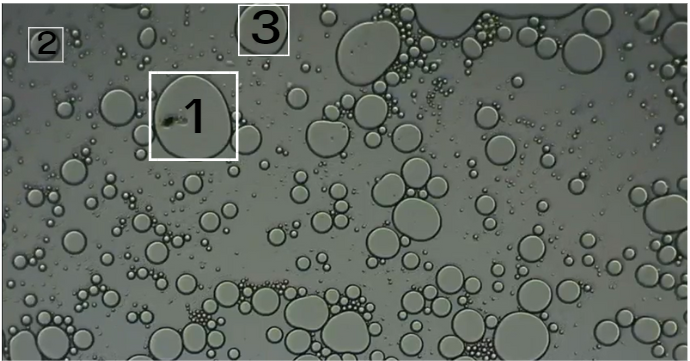
\includegraphics[width=\textwidth]{3_2.png}
  \end{center}
  \caption[Poem]{}
\end{figure}
